\PassOptionsToPackage{dvispnames, table}{xcolor}
\documentclass[aspectratio=169, onlytextwidth]{beamer}
\usetheme[institute]{tugraz2018}
\usepackage[beamer]{prettytex/base}
\usepackage{prettytex/math}
\usepackage{prettytex/gfx}
\usepackage{tabularray}
\usepackage{neuralnetwork}
\usepackage{cancel}
\usepackage{braket}
\usepackage[nameinlink]{cleveref}

\setlength{\headheight}{19.53pt}
\setlength{\headsep}{1.8em}
\setlength{\belowcaptionskip}{-12pt}

\makeatletter
\renewcommand\listoffigures{
  \section*{\listfigurename}
  \@starttoc{lof}
}
\renewcommand\listoftables{
  \section*{\listtablename}
  \@starttoc{lot}
}
\makeatother

\crefname{figure}{figure}{figures}
\crefname{tcb@cnt@definition}{definition}{definitions}
\crefname{tcb@cnt@theorem}{theorem}{theorems}
\crefname{tcb@cnt@lemma}{lemma}{lemmata}
\crefname{tcb@cnt@corollary}{corollary}{corollaries}
\crefname{tcb@cnt@remark}{remark}{remarks}


\tikzexternalize[prefix=tikz/]
\renewcommand{\inputtikz}[1]{
  \tikzsetnextfilename{#1}
  \input{../thesis/#1.tex}
}

\title[Secure Classification as a Service]{
  Secure Classification as a Service \\
  \small\normalfont\textcolor{black}{
    Levelled Homomorphic, Post-Quantum Secure Machine Learning Inference \\
    based on the CKKS Encryption Scheme
  }
}
\author{Peter Waldert}
\date{Bachelor Thesis Presentation, 01.08.2022}
\institute{IAIK}
\instituteurl{iaik.tugraz.at}

\institutelogo{beamerthemetugraz/institute/IAIK}
% \additionallogo{figures/logo}  % additional institute/department logo (footline; optional)
% \logobar{Supported by: ...}  % sponsors (titlepage; optional)

% Ungefähre Struktur:
% * Motivation aus zwei Richtungen: Privacy-Preserving Machine Learning möglich? (Anwendungen in der Medizin) -> HE
%   netter Side-Effect: Post-Quantum Security via Lattice Cryptography
% * Beispiel für HE und Public-Key Asymmetric Encryption zur Veranschaulichung: RSA
% * Learning With Errors und andere Lattice Probleme (nur ein paar Sätze)
% * Relation von CKKS zu LWE: Wie der Private Key geschützt ist und Hardness des LWE-Problems.
% * CKKS Scheme erklären, dazu: Polynomring Z_q[X]/(X^N+1) erläutern, wie wird encoded und verschlüsselt
% * Zeigen, dass Encrypt(Encode(z)) + Encrypt(Encode(z')) == Encrypt(Encode(z + z')) in CKKS
% * Implementation erklären (SEAL, Struktur in Server/Client, etc.), Demo der UI.
% * Verschiedene Matmul-Implementationen, Optimierungen
% * Ergebnisse: Performance des Netzwerks, Benchmarks, Ciphertext-Visualisierungen.

\setlength{\headheight}{19.53pt}

\makenoidxglossaries
\newacronym{he}{HE}{Homomorphic Encryption}
\newacronym{fhe}{FHE}{Fully Homomorphic Encryption}
\newacronym{bfv}{BFV}{Brakerski-Fan-Vercauteren}
\newacronym{bgv}{BGV}{Brakerski-Gentry-Vaikuntanathan}
\newacronym{ckks}{CKKS}{Cheon-Kim-Kim-Song}
\newacronym{rsa}{RSA}{Rivest-Shamir-Adleman}
\newacronym{aes}{AES}{Advanced Encryption Standard}
\newacronym{lwe}{LWE}{Learning With Errors}
\newacronym{dlwe}{DLWE}{Decision Learning With Errors}
\newacronym{rlwe}{RLWE}{Learning With Errors on Rings}
\newacronym{tls}{TLS}{Transport Layer Security}
\newacronym{ml}{ML}{Machine Learning}
\newacronym{gd}{GD}{Gradient Descent}
\newacronym{mse}{MSE}{Mean-Squared-Error}
\newacronym{dft}{DFT}{Discrete Fourier Transform}
\newacronym{fft}{FFT}{Fast Fourier Transform}
\newacronym{iff}{iff}{if and only if}
\newacronym{np}{NP}{Non-deterministic Polynomial time}
\newacronym{ppml}{PPML}{Privacy-Preserving Machine Learning}
\newacronym{mnist}{MNIST}{Modified National Institute of Standards and Technology database}
\newacronym{sis}{SIS}{Shortest Integer Solution}
\newacronym{svp}{SVP}{Shortest Vector Problem}
\newacronym{gapsvp}{GapSVP}{Decisional Approximate Shortest Vector Problem}
\newacronym{fhew}{FHEW}{Fastest Homomorphic Encryption in the West}
\newacronym{tfhe}{TFHE}{Torus Fully Homomorphic Encryption}
\newacronym{crt}{CRT}{Chinese Remainder Theorem}
\newacronym{rns}{RNS}{Residue Number System}

\newcommand{\cpp}[1]{\mintinline{cpp}{#1}}
\newcommand{\name}[1]{\textsc{#1}}
\newcommand{\cryptop}[1]{\text{\textcolor{darkpurple}{#1}}}
\newcommand{\inv}{^{-1}}
\newcommand{\inputtikz}[1]{
  % \tikzsetnextfilename{#1}
  % \input{#1.tex}
  \vspace{2cm}
  Placeholder
  \vspace{2cm}
}

\addbibresource{../library/sources.bib}

\begin{document}
  \begin{frame}[plain]
    \maketitle
  \end{frame}

  \begin{frame}{Outline}
    \tableofcontents
  \end{frame}

  \chapter{Introduction}
\label{chap:introduction}
The most well-known and widely used asymmetric ('public-key') cryptographic scheme, published by the trio \name{Rivest}-\name{Shamir}-\name{Adleman} in 1977 and known as \textit{RSA}, is based on the hardness assumption of the integer factorisation problem (factorising a large 2-composite number into its two prime factors $p$ and $q$ is hard).
As of today, this factorisation problem has not been proven to be in NP, yet it is suspected that it might indeed be NP-complete (i.e. \hyperref[def:np-hard]{NP-hard} while still being in NP) when modelled using a traditional Turing machine.
Since the advent of quantum computation, this situation changed as a whole with Peter \name{Shor}'s algorithm, threatening the security of many cryptosystems, for instance RSA which is still widely used today despite its known problems.

As it stands, lattice-based cryptography presents a solution to a politically and socially problematic situation in which few parties world-wide, with access to a sufficiently powerful quantum computer, may be able to decrypt most of today's digital communication.
\hyperref[subsec:lattice-crypto]{Lattice Cryptography} is based on other mathematical problems, shown to be sufficiently hard on quantum computers and traditional ones alike, most notably \hyperref[def:lwe-search-problem]{LWE} which this thesis will discuss in detail.

Many new cryptosystems have been developed on top of LWE, two of which this following thesis will focus on specifically: \hyperref[def:bfv-scheme]{BFV} and \hyperref[def:ckks-scheme]{CKKS};
whose security is still unaffected by efficient quantum algorithms.
Yet, it is not only their security prospect that makes these encryption schemes attractive, but first and foremost their defining \hyperref[def:ring-homomorphism]{homomorphic} property which allows for computations on the encrypted data.
A \textit{fully} homomorphic encryption (FHE) scheme was first introduced by Craig \name{Gentry} in 2009, using a bootstrapping approach.
The \textit{levelled} homomorphic \gls{bgv} encryption scheme is implemented in Microsoft SEAL and allows for integer arithmetic, up to a few multiplication 'levels' deep.
The \gls{bfv} scheme is very similar to it and described in a bit more detail in \autoref{sec:bfv}.
And finally, building upon concepts introduced in the former, the \gls{ckks} scheme allows for approximative floating-point arithmetic that finally facilitates machine-learning applications.

Machine Learning allows a computer to 'learn' from specifically structured data using linear regression or similar methods, and applying this 'knowledge' to new, unknown inputs.
In its simplest form, or even using a neural network, this only requires two different operations on numbers (or even better, vectors): addition and multiplication.
Using an \gls{he} scheme such as the ones mentioned above and described in \autoref{chap:homomorphic-encryption}, both are given and PPML (Privacy-Preserving Machine Learning) applications are born!

Considering the implications of mass surveilance, the importance of privacy-preserving/enhancing technologies should not be forgotten.

The present thesis not only focusses on theoretical remarks but also includes a publicly available implementation of an \gls{he} classification server written in C++ and a compact graphical user interface to interact with.
The following aims to introduce most of the necessary theory to understand the homomorphic encryption schemes used in practice today, as well as the simple machine learning approaches involved in securely classifying images as a service.

  \section{Step 2: Lattice Cryptography, LWE and RLWE}
\begin{frame}[c]{Lattices}
  \begin{columns}
    \begin{column}{0.32\linewidth}
      \begin{figure}
        \centering
        \scalebox{0.5}{\inputtikz{figures/lattice}}
        % \caption[Illustration of a standard lattice]{
        %   Illustration of a standard lattice $\lat$ with two basis vectors $\vec{b}_1$ and $\vec{b}_2$.
        % }
        \label{fig:lattice}
      \end{figure}
    \end{column}
    \begin{column}{0.6\linewidth}
      \begin{definition}[Lattice]
        A lattice $(\lat, +, \cdot)$ is a vector field over the integers $(\Z, +, \cdot)$, given $n$ basis vectors $\vec{b_1}, \vec{b_2}, ..., \vec{b_n} \in \R^n$, with
        $$\lat := \bigg\{\sum_{i=1}^n c_i \vec{b}_i \,\bigg|\, c \in \Z\bigg\} \subseteq \R^n \,.$$
      \end{definition}
    \end{column}
  \end{columns}
\end{frame}

\begin{frame}{The \gls{lwe} Problem}
  \begin{definition}[LWE-Distribution $A_{\vec{s}, \chi_{error}}$]
    Given a prime $q \in \N$ and $n \in \N$, choose a secret $\vec{s} \in (\Z / q \Z)^n$.
    Sampling from $A_{\vec{s}, \chi_{error}}$:
    \begin{itemize}
      \item Sample a uniformly random vector $a \in (\Z/q\Z)^n$.
      \item Sample a scalar 'error term' $\mu \in \Z / q \Z$ from $\chi_{error}$.
      \item Compute a noisy inner product $b = \vec{s} \cdot \vec{a} + \mu$.
      \item Output the pair $(\vec{a}, b) \in (\Z / q \Z)^n \times (\Z / q \Z)$.
    \end{itemize}
  \end{definition}

  Search-LWE-Problem:
  Given $m$ independent samples $(\vec{a}_i, b_i)_{0 < i \leq m}$ from $A_{\vec{s}, \chi_{error}}$, find $\vec{s}$.

  Published by \name{Regev} in 2005 \cite{2005-lwe-original}.
  Lead to the \glstext{fhe} scheme by \name{Gentry} in 2009 \cite{2009-gentry-fhe-original}.
\end{frame}

\begin{frame}{What is CKKS?}
  \begin{itemize}
    \item Levelled Homomorphic Encryption Scheme \cite{2017-ckks-original}.
          $$\forall m_1, m_2: \mathcal{E}(m_1) + \mathcal{E}(m_2) = \mathcal{E}(m_1 + m_2) \text{ and } \mathcal{E}(m_1) \cdot \mathcal{E}(m_2) = \mathcal{E}(m_1 \cdot m_2)$$
    \item Enables Public-Key (Asymmetric) Cryptography.
    \item Approximative Floating-Point Arithmetic.
    \item Security based on \glsdesc{lwe}.
    \item \gls{simd} Encoding.
  \end{itemize}
\end{frame}

\begin{frame}{Overview of \gls{ckks}}
  \begin{figure}[H]
    \centering
    \scalebox{0.85}{\inputtikz{figures/ckks-schematic}}
    % \caption[Schematic overview of the CKKS scheme]{
    %   Schematic overview of CKKS \parencite{2017-ckks-original}, adapted from \cite{2020-cryptotree}.
    %   A plain vector $\vec{z} \in \C^{N/2}$ is encoded to $m = \cryptop{CKKS.Encode}(\vec{z})$, encrypted to $\vec{c} = \cryptop{CKKS.Encrypt}(\vec{p}, m)$, decrypted and decoded to a new $\tilde{\vec{z}} = \cryptop{CKKS.Decode}(\cryptop{CKKS.Decrypt}(s, \tilde{\vec{c}}))$.
    % }
    \label{fig:ckks-overview}
  \end{figure}
\end{frame}

\begin{frame}{Encryption and Decryption}
  Public key $\vec{p} = (b, a)$ with $b = -(as + \tilde{\mu})$, secret key $s$, probability distributions $\chi_{enc}$, $\chi_{error}$, plaintext (=message) $m \in R/qR$, ciphertext $\vec{c}$.

  \cryptop{CKKS.} \\
  \begin{tblr}{Q[l,h]Q[l,h,\textwidth - 3.5cm]}
    \cryptop{Encrypt}$(\vec{p}, m)$ & {
        Let $(b,a) = \vec{p}$, $u \leftarrow \chi_{enc}$, $\mu_1, \mu_2 \leftarrow \chi_{error}$,
        then the ciphertext is $\vec{c} = u \cdot \vec{p} + (m + \mu_1, \mu_2) = (m + bu + \mu_1, au + \mu_2)$
        $\quad\rightarrow \vec{c}$} \\
    \cryptop{Decrypt}$(s, \vec{c})$ & {
        Decrypt the ciphertext $\vec{c} = (c_0, c_1)$ as $m = \lbrack c_0 + c_1 s\rbrack_{q_L}$
        $\quad\rightarrow m$} \\
  \end{tblr}
  \begin{itemize}
    \item A public-key cryptosystem! Encrypt with $\vec{p}$, decrypt with $s$.
    \item Leaves the attacker with the \gls{rlwe} problem.
  \end{itemize}
\end{frame}

\begin{frame}{Homomorphic Addition}
  \begin{tblr}{Q[l,h]Q[l,h,\textwidth - 3.5cm]}
    \cryptop{CKKS.Add}$(\vec{c}, \vec{c}')$ & {
        Output $\overline{\vec{c}} = \vec{c} + \vec{c}' = \begin{pmatrix}
            \delta (m + m') + b (u + u') + (\mu_1 + \mu_1') \\
            a (u + u') + (\mu_2 + \mu_2')
          \end{pmatrix}^T$} \\
  \end{tblr}

  Indeed, the ciphertext $\overline{\vec{c}}$ correctly decrypts back to $\overline{m} := m + m'$:
  \begin{align*}
    \cryptop{CKKS.Decrypt}(s, \overline{\vec{c}})
     & = \lfloor \delta\inv [\overline{c_0} + \overline{c_1} s]_t \rceil                                                                                                                                                         \\
     & = \big\lfloor \delta\inv [\delta \overline{m} + b \overline{u} + \overline{\mu_1} + (a \overline{u} + \overline{\mu_2}) s]_t \big\rceil                                                                                   \\
     & = \big\lfloor [(\delta\inv\delta) \overline{m} + \delta\inv b \overline{u} + \delta\inv \overline{\mu_1} + \delta\inv a s \overline{u} + \delta\inv \overline{\mu_2} s]_t \big\rceil                                      \\
     & = \big\lfloor [\overline{m} - \cancel{\delta\inv as \overline{u}} - \delta\inv \tilde{\mu} \overline{u} + \delta\inv \overline{\mu_1} + \cancel{\delta\inv as \overline{u}} + \delta\inv \overline{\mu_2} s]_t \big\rceil \\
     & = \big\lfloor [\overline{m} + \underbrace{\delta\inv (\overline{\mu_1} + \overline{\mu_2} s - \tilde{\mu} \overline{u})}_{:= \epsilon \,, ||\epsilon|| \ll 1}]_t \big\rceil
    \approx \big\lfloor [\overline{m}]_t \big\rceil = \lfloor \overline{m} \rceil \approx \overline{m}
  \end{align*}
\end{frame}

  \section{The CKKS Scheme}
\begin{frame}{Overview of \gls{ckks}}
  \begin{figure}[H]
    \centering
    \scalebox{0.8}{\inputtikz{figures/ckks-schematic}}
    \caption[Schematic overview of the CKKS scheme]{
      Schematic overview of CKKS \parencite{2017-ckks-original}, adapted from \cite{2020-cryptotree}.
      A plain vector $\vec{z} \in \C^{N/2}$ is encoded to $m = \cryptop{CKKS.Encode}(\vec{z})$, encrypted to $\vec{c} = \cryptop{CKKS.Encrypt}(\vec{p}, m)$, decrypted and decoded to a new $\tilde{\vec{z}} = \cryptop{CKKS.Decode}(\cryptop{CKKS.Decrypt}(s, \tilde{\vec{c}}))$.
    }
    \label{fig:ckks-overview}
  \end{figure}
\end{frame}

\begin{frame}{Encoding and Decoding}
  \cryptop{CKKS.} \\
  \begin{tblr}{Q[l,h]Q[l,h,\textwidth - 3.5cm]}
    \cryptop{Encode}$(\vec{z})$ & {For a given input vector $\vec{z}$, output
        $m = (\underline{\sigma}\inv \circ \underline{\rho_\delta}\inv \circ \underline{\pi}\inv)(\vec{z}) = \underline{\sigma}\inv(\lfloor \delta \cdot \underline{\pi}\inv(\vec{z})\rceil_{\underline{\sigma}(R)})$ $\quad\rightarrow m$} \\
    \cryptop{Decode}$(m)$ & {Decode plaintext $m$ as
        $\vec{z} = (\underline{\pi} \circ \underline{\rho_\delta} \circ \underline{\sigma})(m) = (\underline{\pi} \circ \underline{\sigma})(\delta\inv m)$
        $\quad\rightarrow \vec{z}$} \\
  \end{tblr}
  \begin{itemize}
    \item Three transformations: $\underline{\sigma}\inv$, $\underline{\rho_\delta}\inv$ and $\underline{\pi}\inv$.
    \item Key idea: Homomorphic property, they preserve additivity and multiplicativity.
    \item Allows for homomorphic \gls{simd} operations.
  \end{itemize}
\end{frame}

\begin{frame}{Encryption and Decryption}
  \cryptop{CKKS.} \\
  \begin{tblr}{Q[l,h]Q[l,h,\textwidth - 3.5cm]}
    \cryptop{Encrypt}$(\vec{p}, m)$ & {
        Let $(b,a) = \vec{p}$, $u \leftarrow \chi_{enc}$, $\mu_1, \mu_2 \leftarrow \chi_{error}$,
        then the ciphertext is $\vec{c} = u \cdot \vec{p} + (m + \mu_1, \mu_2) = (m + bu + \mu_1, au + \mu_2)$
        $\quad\rightarrow \vec{c}$} \\
    \cryptop{Decrypt}$(s, \vec{c})$ & {
        Decrypt the ciphertext $\vec{c} = (c_0, c_1)$ as $m = \lbrack c_0 + c_1 s\rbrack_{q_L}$
        $\quad\rightarrow m$} \\
  \end{tblr}
  \begin{itemize}
    \item A public-key cryptosystem! Encrypt with $\vec{p}$, decrypt with $s$.
    \item Leaves the attacker with the \gls{rlwe} problem.
    \item Decrypts correctly under certain conditions...
  \end{itemize}
\end{frame}

\begin{frame}{Homomorphic Addition}
  \begin{tblr}{Q[l,h]Q[l,h,\textwidth - 3.5cm]}
    \cryptop{CKKS.Add}$(\vec{c}, \vec{c}')$ & {
        Output $\overline{\vec{c}} = \vec{c} + \vec{c}' = \begin{pmatrix}
            \delta (m + m') + b (u + u') + (\mu_1 + \mu_1') \\
            a (u + u') + (\mu_2 + \mu_2')
          \end{pmatrix}^T$} \\
  \end{tblr}

  Indeed, the ciphertext $\overline{\vec{c}}$ correctly decrypts back to $\overline{m} := m + m'$:
  \begin{align*}
    \cryptop{CKKS.Decrypt}(s, \overline{\vec{c}})
     & = \lfloor \delta\inv [\overline{c_0} + \overline{c_1} s]_t \rceil                                                                                                                                                         \\
     & = \big\lfloor \delta\inv [\delta \overline{m} + b \overline{u} + \overline{\mu_1} + (a \overline{u} + \overline{\mu_2}) s]_t \big\rceil                                                                                   \\
     & = \big\lfloor [(\delta\inv\delta) \overline{m} + \delta\inv b \overline{u} + \delta\inv \overline{\mu_1} + \delta\inv a s \overline{u} + \delta\inv \overline{\mu_2} s]_t \big\rceil                                      \\
     & = \big\lfloor [\overline{m} - \cancel{\delta\inv as \overline{u}} - \delta\inv \tilde{\mu} \overline{u} + \delta\inv \overline{\mu_1} + \cancel{\delta\inv as \overline{u}} + \delta\inv \overline{\mu_2} s]_t \big\rceil \\
     & = \big\lfloor [\overline{m} + \underbrace{\delta\inv (\overline{\mu_1} + \overline{\mu_2} s - \tilde{\mu} \overline{u})}_{:= \epsilon \,, ||\epsilon|| \ll 1}]_t \big\rceil
    \approx \big\lfloor [\overline{m}]_t \big\rceil = \lfloor \overline{m} \rceil \approx \overline{m}
  \end{align*}
\end{frame}

  \chapter{Implementation}
\label{chap:implementation}

\section{Chosen Software Architecture}
In the given setting, the most accessible frontend is commonly a JavaScript web application.

To still make the classification run as quickly and efficiently as possible, a C++ binary runs
in the backend providing an HTTP API to the frontend application.
In order to allow for more flexibility of the HTTP server, the initial approach was to
pipe requests through a dedicated web application framework with database access
that would allow, for instance, user management next to the basic classification.
However, the resulting communication and computation overhead, even when running with very
efficient protocols such as ZeroMQ, was too high.

Extending the accessibility argument to reproducibility, Docker is a very solid choice \parencite{using-docker-in-science}.
To run the attached demo project, simply execute
\begin{minted}{bash}
  docker-compose build
  docker-compose up
\end{minted}
in the 'code' folder and point your browser to \url{https://localhost}.

\subsection{Docker Multi-Stage Build}
An enterprise-grade, scalable deployment is achieved by means of zero-dependency
Alpine Linux images which contain nothing but compiled binaries and linked libraries.


\section{The MNIST dataset}
The MNIST dataset \parencite{mnist-original} contains X train and Y test images with corresponding labels.
In order to stick to the traditional feedforward technique with data represented
in vector format, therefore it is common to reshape data from $(28, 28)$ images (represented as grayscale values in a matrix)
into a $784$ element vector.

\section{Matrix-Vector Multiplication}
The dot product that is required as part of the neural network evaluation process
needs to be implemented on SEAL ciphertexts as well.

There are multiple methods to achieve a syntactically correct dot product (matrix-vector multiplication)
as described by \textcite{2018-gazelle} for square matrices.

\begin{enumerate}
  \item Naive
  \item Diagonal
  \item Hybrid
  \item Babystep-Giantstep
\end{enumerate}

\begin{figure}
  \centering
  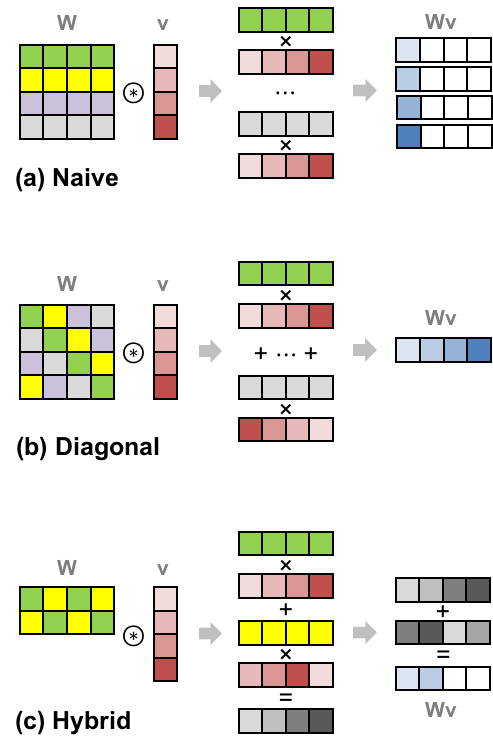
\includegraphics[width=0.4\linewidth]{figures/matrix-vector-multiplication-techniques.png}
  \caption[Image source: \cite{2018-gazelle}]{Different techniques to compute a dot product between a matrix and a vector,
    each having their up- and downsides.}
\end{figure}

\subsection{Adapting to non-square matrices}
The weight matrices in the given classification setting
are by no means square, on the contrary their output dimension tends
to be much lower than the input dimension as the goal is to reduce it from
$28^2 = 784$ to $10$ overall.

However, that also means one cannot directly apply the diagonal method
as described in the proceedings above.
This 'flaw' can be mitigated by a simple zero-padding approach
in order to make the matrix square, filling in zeros until
the lower dimension reaches the higher one.

\subsection{The Naive Method}
Term by term, one can express a matrix-vector product as follows:
$$\{M \vec{x}\}_i = \sum_{j=1}^{t} M_{ij} x_j$$

\subsection{The Diagonal Method}
For the following, define
\newcommand{\rot}{\mathrm{rot}}
\newcommand{\diag}{\mathrm{diag}}
$$\rot_j: \R^t \mapsto \R^t, \; \{\rot_j(\vec{x})\}_i = x_{i + j}$$
$$\diag_j: \R^{t \times t} \mapsto \R^t, \; \{\diag_j(M)\}_i = M_{i, (i+j)}$$
with all indices $i, j \in \Z_t$ member of the cyclic quotient group $\Z_t := \Z / t \Z$ of all integers
modulo $t$, meaning that overflowing indices simply wrap around again starting at index $0$ to simplify notation.
For the sake of compactness, we stick to this notation for the rest of this section.

\subsection{The Hybrid Method}
\subsection{The Babystep-Giantstep Optimization}
Since Galois rotations are the most computationally intensive operations in most cryptographic schemes used
today \parencite{2021-pasta}, they take a large toll on the efficiency.
In order to reduce the number of rotations required, one can make use of the \textit{Babystep-Giantstep}
optimization as described in \cite{2018-faster-helib}, which works as follows:

\begin{theorem}{Babystep-Giantstep Optimization}{bsgs}
  Given a matrix $M \in \R^{t \times t}$ and a vector $\vec{x} \in \R^t$,
  with $t = t_1 \cdot t_2$ split into two BSGS parameters $t_1, t_2 \in \N$ and
  $$\diag'_p(M) = \rot_{-\lfloor p/t_1 \rfloor \cdot t_1}(\diag_p(M))$$,
  one can express a matrix-vector multiplication as follows:
  \begin{equation}
    M \vec{x} = \sum_{k=0}^{t_2-1} \rot_{(kt_1)} \bigg(
    \sum_{j=0}^{t_1-1} \diag'_{(kt_1+j)}(M) \cdot \rot_j(\vec{x})
    \bigg)
  \end{equation}
  where $\cdot$ denotes an element-wise multiplication of two vectors.
\end{theorem}

\begin{proof}
  Starting from the adapted matrix-multiplication expression $P = (P_1, P_2, ..., P_t)^T \in \R^t$,
  we want to show that we indeed end up with an authentic matrix-vector product.
  \begin{align*}
    P = \bigg\{\sum_{k=0}^{t_2-1} \rot_{(kt_1)} \big(
    \sum_{j=0}^{t_1-1} \diag'_{(kt_1+j)}(M) \cdot \rot_j(\vec{x})
    \big)\bigg\}_i = \sum_{k=0}^{t_2-1} \sum_{j=0}^{t_1-1} m'_{kt_1+j,(i+kt_1)} x_{(i+kt_1)+j}
  \end{align*}
  with
  \begin{align*}
    m'_{p,i} = \big\{ diag'_p(M)\big \}_i = \big\{ \rot_{-\lfloor p/t_1 \rfloor \cdot t_1}(\diag_p(M)) \big\}_i
    = M_{i-\lfloor\frac{p}{t_1}\rfloor t_1, i-\lfloor\frac{p}{t_1}\rfloor t_1 + p}
  \end{align*}
  and therefore
  \begin{align*}
    m'_{kt_1+j,i}        & = M_{i-\lfloor\frac{kt_1+j}{t_1}\rfloor t_1, i-\lfloor\frac{kt_1+j}{t_1}\rfloor t_1 + kt_1+j} \\
                         & = M_{i-kt_1-\lfloor\frac{j}{t_1}\rfloor t_1, i-kt_1-\lfloor\frac{j}{t_1}\rfloor t_1 + kt_1+j} \\
                         & = M_{i-kt_1-\lfloor\frac{j}{t_1}\rfloor t_1, i+j-\lfloor\frac{j}{t_1}\rfloor t_1}             \\
    m'_{kt_1+j,(i+kt_1)} & = M_{i+kt_1-kt_1-\lfloor\frac{j}{t_1}\rfloor t_1, i+kt_1+j-\lfloor\frac{j}{t_1}\rfloor t_1}   \\
                         & = M_{i-\lfloor\frac{j}{t_1}\rfloor t_1, i+kt_1+j-\lfloor\frac{j}{t_1}\rfloor t_1}
  \end{align*}
  leading to
  \begin{align*}
    P_i = \sum_{k=0}^{t_2-1} \sum_{j=0}^{t_1-1} m'_{kt_1+j,(i+kt_1)} x_{(i+kt_1)+j}
    = \sum_{k=0}^{t_2-1} \sum_{j=0}^{t_1-1} M_{i-\lfloor\frac{j}{t_1}\rfloor t_1, i+kt_1+j-\lfloor\frac{j}{t_1}\rfloor t_1} x_{(i+kt_1)+j}
  \end{align*}
  . Noticing that the downward rounded fraction $\lfloor\frac{j}{t_1}\rfloor$ vanishes
  in a sum with $j$ running from $0$ to $t_1-1$, we can simplify to
  \begin{align*}
    P_i = \sum_{k=0}^{t_2-1} \sum_{j=0}^{t_1-1} M_{i,i+kt_1+j} x_{i+kt_1+j}
  \end{align*}
  which contains two sums running to $t_1$ and $t_2$ respectively, containing an expression
  of the form $k \cdot t_1 + j$, which allows us to condense the nested sums into one single
  summation expression, as $$\sum_{k=0}^{t_2-1} \sum_{j=0}^{t_1-1} f(kt_1+j) = \sum_{l=0}^{t-1} f(l)$$
  indeed catches every single value $l \in \{0, 1, 2, ..., t=t_1 \cdot t_2\}$ with $l = kt_1+j$. \\
  In summary, we obtain
  \begin{align*}
    P_i & = \sum_{k=0}^{t_2-1} \sum_{j=0}^{t_1-1} M_{i,i+kt_1+j} x_{i+kt_1+j} \\
        & = \sum_{l=0}^{t-1} M_{i,i+l} x_{i+l}
    = \sum_{\nu=0}^{t-1} M_{i,\nu} x_{\nu}                                    \\
        & = \big\{M \vec{x}\big\}_i
  \end{align*}
  which indeed equals the conventional definition of a matrix-vector product.
\end{proof}

Note that the optimized matrix-vector multiplication only requires $t_1 + t_2$ as
we can store the $t_1$ inner rotations of the vector $x$ for the upcoming evaluations.
For larger matrices and vectors (larger $t$), $t_1 + t_2$ are indeed much smaller than
the conventional number of required rotations in the Diagonal or Hybrid method for instance
which was the point of this modification in the first place.

\section{Polynomial Evaluation}
From the implementation perspective, there are three properties to watch out for when
working with SEAL ciphertexts:

\begin{enumerate}
  \item Scale (retrieved using \cpp{x.scale()})
        \begin{quote}
          Scale has nothing to do with noise. "Scale out of bounds" can appear even if noise is extremely low. Although repeated multiplication of a ciphertext by a plaintext will slowly increase the noise, it is not the reason why you see "scale out of bounds".
          "Scale out of bounds" error specifically means that the scale of a ciphertext or plaintext is larger than the product of all elements in coeff\_modulus. If you perform multiplications without rescaling, you can quickly see this error. The more rescaling you perform, the less elements will be left in coeff\_modulus. Even if you managed to have the same scale in a ciphertext after every multiplication and rescale, eventually the coeff\_modulus can be too small to accommodate another multiplication.
        \end{quote}
        % https://github.com/microsoft/SEAL/issues/182#issuecomment-646234787

        Can be adjusted with: \cpp{evaluator.rescale_inplace()}
  \item Encryption Parameters (retrieved using \cpp{x.parms_id()}) \\
        Can be adjusted with: \cpp{evaluator.mod_switch_to_inplace()}
  \item Ciphertext Size (retrieved using \cpp{x.size()}) \\
        Can be adjusted with: \cpp{evaluator.relinearize_inplace()}
\end{enumerate}

\paragraph{Multiplication}
Each time one multiplies two ciphertexts, the scales multiply (logarithmically, they add up, i.e. the bits are added together).
The chain index reduces by 1. The chain index of an encoded ciphertext depends on the coeff moduli.
There must be enough bits remaining to perform the multiplication, namely log2(scale) bits.

\paragraph{Addition}
The scales must be the same, but luckily they will not change.

\section{Transparent Ciphertext}
\begin{quote}
  The problem is that you are subtracting a ciphertext from itself.
  This kind of operation results in a ciphertext that is identically zero;
  this is called a transparent ciphertext. Such a transparent ciphertext
  is not considered to be valid because the ciphertext reveals its underlying plaintext to anyone who sees it,
  even if they don't have the secret key.
  By default SEAL throws an exception when such a situation is encountered to protect you from a problem you may not have noticed.
  If you truly know what you are doing and want to enable the creation of transparent ciphertexts,
  you can configure SEAL [...].
  \parencite{kim-laine-on-transparent-ciphertexts}
\end{quote}

% https://github.com/microsoft/SEAL/issues/276#issuecomment-777073477
'transparent ciphertexts (a.k.a. ciphertexts whose second polynomial is zero) are malformed and do not need the secret key to decrypt'


  \section{Live Demo of the WebApp}
  \begin{frame}{Demo: Secure Handwritten Digit Classification as a Service}
    \begin{columns}[c]
      \begin{column}{0.7\linewidth}
        \begin{figure}[H]
          \centering
          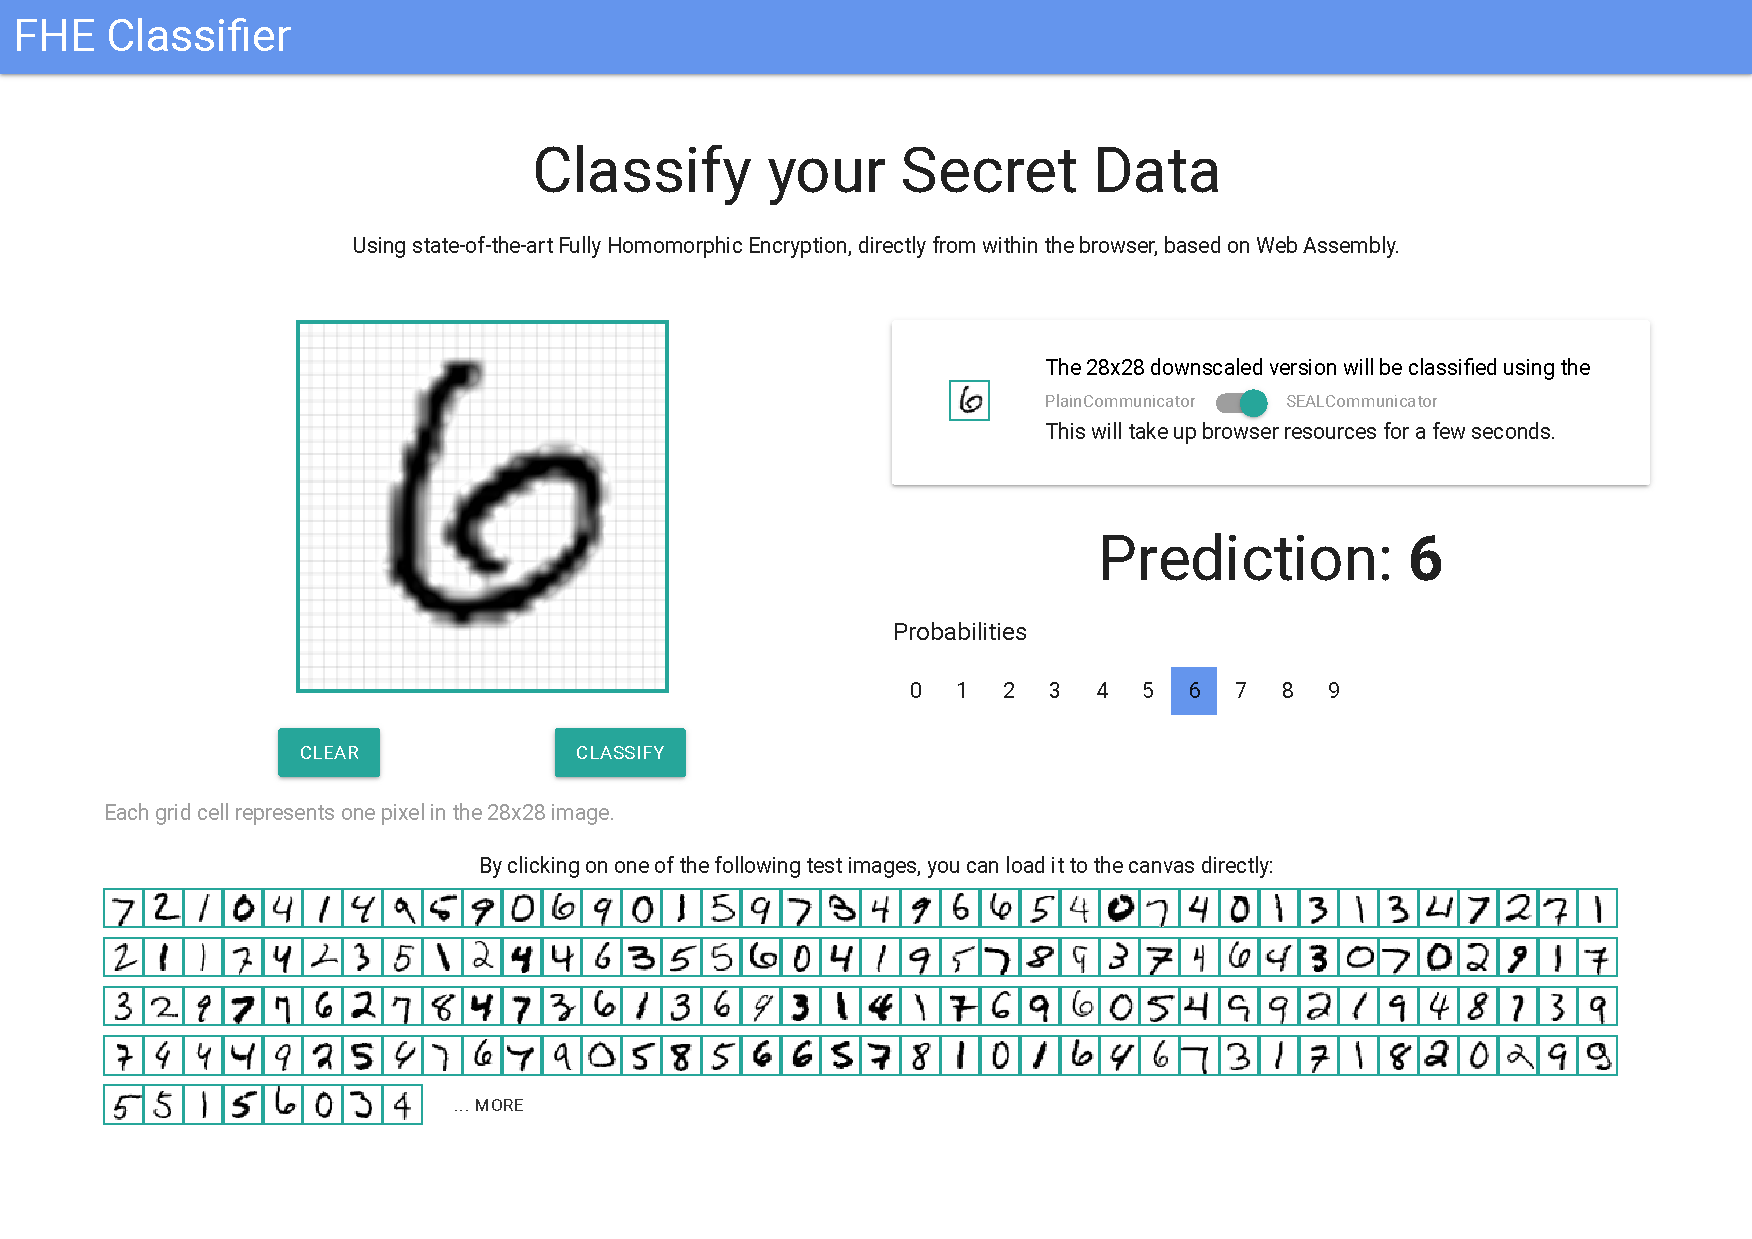
\includegraphics[width=0.75\linewidth]{../thesis/figures/frontend.pdf}
          \vspace{-0.3cm}
          \caption{\url{https://secure-classification.peter.waldert.at/}.}
        \end{figure}
      \end{column}
      \begin{column}{0.24\linewidth}
        Scan the QR-Code:
        \qrcode[nolink,height=3.1cm]{https://secure-classification.peter.waldert.at/}
      \end{column}
    \end{columns}
  \end{frame}

  \section{Step 5: Results and Accuracy}
\begin{frame}{Chaos everywhere: The Confusion Matrix}
  \centering
  \scalebox{0.64}{\inputtikz{figures/generated/confusion-matrix}}

  \vspace{-0.3cm}
  Plain Accuracy: \SI{97.6}{\percent}, Encrypted Accuracy: \SI{97.3}{\percent}.
\end{frame}

\begin{frame}{Ciphertext Visualisations}
  \begin{figure}[H]
    \centering
    \scalebox{0.9}{\inputtikz{figures/ciphertext-visualisation}}
    % \caption[Visualisation of the plain input images compared to their ciphertext]{Ciphertext Visualisation: The first row corresponds to the images in plain, the second row depicts an encrypted version, namely the reconstructed polynomial coefficients $\{a_k\}$ of the ciphertext polynomial.}
    \label{fig:ciphertext-visualisation}
  \end{figure}
\end{frame}


  \section*{}
  \begin{frame}{Conclusion}
    \begin{itemize}
      \item Schemes like \gls{rsa} become problematic due to \name{Shor}'s Algorithm $\Rightarrow$ Lattice Crypto.
      \item New Cryptosystems constructed based on \name{Regev}'s \gls{lwe}-problem, e.g. \gls{ckks}.
      \item Encryption is homomorphic with respect to addition (and multiplication).
      \item The Encoding and Decoding procedures of CKKS allow for \gls{simd} operations needed for efficient computations.
      \item Image Classification of the handwritten digits can be done using a neural network.
      \item The required operations can be translated to \gls{he}.
      \item For better performance, improved matrix multiplication methods are utilised.
      \item Our Demonstrator: \url{https://secure-classification.peter.waldert.at/}.
    \end{itemize}
  \end{frame}

  %\begin{frame}[c,plain]
  \begin{frame}[c]
    \centering
    \Large Questions?
  \end{frame}

  \begin{frame}[allowframebreaks]{Glossary}
    \printnoidxglossary[type=acronym]
  \end{frame}

  \begin{frame}[allowframebreaks]{Bibliography}
    \printbibliography
  \end{frame}

  \appendix
\titleformat{\chapter}[block]{\normalfont\LARGE\bfseries}{Appendix \thechapter \;\textendash\;}{0ex}{\vspace{-4cm}}[\vspace{4.5cm}]
\titlespacing{\chapter}{0cm}{0cm}{0cm}

\chapter{Supplemental Proofs}
\label{chap:appendix}

\section{Power-of-2 Cyclotomic Polynomials}
\label{proof:power-of-2-cyclo-poly}
\begin{proof}[Proof of \cref{thm:power-of-2-cyclo-poly}]
  With $k \in \N$ a positive integer, we want to show that
  $$\Phi_{2^k} (x) = x^{2^{k-1}} + 1\,.$$

  A polynomial $p \in \Z[X]$ with $$p(x) = x^n - a$$ of degree $n$ has $n$ roots
  $$\{x_j\} = \{a^\frac{1}{n} e^{2\pi i \frac{j}{n}} \,|\, j \in \N, j \leq n\}$$
  related by a factor $a^\frac{1}{n}$ to the \hyperref[lemma:nth-roots-of-unity]{$n$\textsuperscript{th} roots of unity} given by powers of $\xi = e^{2\pi i \frac{1}{n}}$.

  It is clear from the fundamental theorem of algebra that the polynomial $p$ with roots $\{x_j\}$ can be factorised as
  $$p(x) = \prod_{j=1}^{n} (x - x_j) = \prod_{j=1}^{n} (x - a^\frac{1}{n} e^{2\pi i \frac{j}{n}})\,.$$

  Fixing $a = -1$, we obtain $p(x) = x^n + 1$ with roots given by
  $$x_j = (-1)^\frac{1}{n} e^{2\pi i \frac{j}{n}}
    = (e^{i\pi})^\frac{1}{n} e^{2\pi i \frac{j}{n}}
    = e^{\frac{i\pi (2j + 1)}{n}}$$
  and according factorisation
  $$p(x) = \prod_{j=1}^{n} (x - e^{\frac{i\pi}{n} (2j + 1)})\,.$$

  Further letting $n = 2^{k-1}$ and observing that
  $$\gcd(2^k, l) = \begin{cases}
      1 & \text{if } l \text{ odd}  \\
      2 & \text{if } l \text{ even}
    \end{cases} \quad l, k \in \N$$
  since a number $2^k$ that can only be decomposed into multiples of $2$
  never shares a factor with an odd number, in accordance with \cref{lemma:nth-roots-of-unity}
  we can conclude that the set of all odd roots of unity is exactly the set of all primitive roots (satisfying $\gcd(2^k, l) = 1$).

  Following from above,
  \begin{align*}
    p(x) = \prod_{j=1}^{2^{k-1}} (x - e^{\frac{i\pi}{n} (2j + 1)})
    = \prod_{\stackrel{l=1}{l \text{ odd}}}^{2^k} (x - e^{\frac{i\pi}{n} l})
    = \prod_{\stackrel{l=1}{\xi^l \text{ primitive}}}^{2^k} (x - \xi^l)
    = \Phi_{2^k}(x)
  \end{align*}
  we arrive exactly at the definition of a cyclotomic polynomial (\cref{def:cyclotomic-poly}). \\
  \parencite{power-of-2-cyclo-poly}
\end{proof}

\section{Babystep-Giantstep Multiplication}
\label{proof:bsgs-matmul}
\begin{proof}[Proof of \cref{thm:bsgs}]
  Starting from the adapted \gls{bsgs} matrix-multiplication result $P = (P_1, P_2, ..., P_t)^T \in \R^t$, we want to show that we indeed end up with an authentic matrix-vector product.
  \begin{align*}
    P_i := \bigg\{\sum_{k=0}^{t_2-1} \rot_{(kt_1)} \big(
    \sum_{j=0}^{t_1-1} \diag'_{(kt_1+j)}(M) \cdot \rot_j(\vec{x})
    \big)\bigg\}_i = \sum_{k=0}^{t_2-1} \sum_{j=0}^{t_1-1} m'_{kt_1+j,(i+kt_1)} x_{(i+kt_1)+j}
  \end{align*}
  with
  \begin{align*}
    m'_{p,i} = \big\{ \diag'_p(M)\big \}_i = \big\{ \rot_{-\lfloor p/t_1 \rfloor \cdot t_1}(\diag_p(M)) \big\}_i
    = M_{i-\lfloor\frac{p}{t_1}\rfloor t_1, i-\lfloor\frac{p}{t_1}\rfloor t_1 + p}
  \end{align*}
  and therefore
  \begin{align*}
    m'_{kt_1+j,i}        & = M_{i-\lfloor\frac{kt_1+j}{t_1}\rfloor t_1, i-\lfloor\frac{kt_1+j}{t_1}\rfloor t_1 + kt_1+j} \\
                         & = M_{i-kt_1-\lfloor\frac{j}{t_1}\rfloor t_1, i-kt_1-\lfloor\frac{j}{t_1}\rfloor t_1 + kt_1+j} \\
                         & = M_{i-kt_1-\lfloor\frac{j}{t_1}\rfloor t_1, i+j-\lfloor\frac{j}{t_1}\rfloor t_1}             \\
    m'_{kt_1+j,(i+kt_1)} & = M_{i+kt_1-kt_1-\lfloor\frac{j}{t_1}\rfloor t_1, i+kt_1+j-\lfloor\frac{j}{t_1}\rfloor t_1}   \\
                         & = M_{i-\lfloor\frac{j}{t_1}\rfloor t_1, i+kt_1+j-\lfloor\frac{j}{t_1}\rfloor t_1}
  \end{align*}
  leading to
  \begin{align*}
    P_i = \sum_{k=0}^{t_2-1} \sum_{j=0}^{t_1-1} m'_{kt_1+j,(i+kt_1)} x_{(i+kt_1)+j}
    = \sum_{k=0}^{t_2-1} \sum_{j=0}^{t_1-1} M_{i-\lfloor\frac{j}{t_1}\rfloor t_1, i+kt_1+j-\lfloor\frac{j}{t_1}\rfloor t_1} x_{(i+kt_1)+j} \,.
  \end{align*}
  Noticing that the downward rounded fraction $\lfloor\frac{j}{t_1}\rfloor$ vanishes
  in a sum with $j$ running from $0$ to $t_1-1$, we can simplify to
  \begin{align*}
    P_i = \sum_{k=0}^{t_2-1} \sum_{j=0}^{t_1-1} M_{i,i+kt_1+j} x_{i+kt_1+j}
  \end{align*}
  which contains two sums running to $t_1$ and $t_2$ respectively, containing an expression of the form $k \cdot t_1 + j$, which allows us to condense the nested sums into one single summation expression, as $$\sum_{k=0}^{t_2-1} \sum_{j=0}^{t_1-1} f(kt_1+j) = \sum_{l=0}^{t-1} f(l)$$ indeed catches every single value $l \in \{0, 1, 2, ..., t=t_1 \cdot t_2\}$ with $l = kt_1+j$. \\
  In summary, we obtain
  \begin{align*}
    P_i & = \sum_{k=0}^{t_2-1} \sum_{j=0}^{t_1-1} M_{i,i+kt_1+j} x_{i+kt_1+j} \\
        & = \sum_{l=0}^{t-1} M_{i,i+l} x_{i+l}
    = \sum_{\nu=0}^{t-1} M_{i,\nu} x_{\nu}                                    \\
        & = \big\{M \vec{x}\big\}_i
  \end{align*}
  which indeed equals the conventional definition of a matrix-vector product.
\end{proof}

\end{document}
